% besdoc.tex V1.0, 17 March 2011

\documentclass[times,mee,doublespace,]{besauth2}
%%\documentclass[times,mee,]{besauth}

\newcommand{\journalnamelc}{British Ecological Society}
\newcommand{\journalabb}{British Ecological Society}
\newcommand{\journalclassshort}{BES}
%%\newcommand{\journalname}{British Ecological Society}
\usepackage{epstopdf,comment}

\usepackage{moreverb}

\usepackage[colorlinks,bookmarksopen,bookmarksnumbered,citecolor=red,urlcolor=red]{hyperref}


\usepackage{lineno}

\newcommand\BibTeX{{\rmfamily B\kern-.05em \textsc{i\kern-.025em b}\kern-.08em
T\kern-.1667em\lower.7ex\hbox{E}\kern-.125emX}}

\bibpunct[; ]{(}{)}{;}{}{}{,}

\def\volumeyear{2016}
\def\VOC{VO}

\begin{document}
\runningheads{P.~B.~Conn, D.~L.~Miller, D.~S.~Johnson, et al.}{Multistate mark-recapture mixture models}

\papertype{Article}

\title{Using multistate mark-recapture mixture models to estimate latent subpopulation structure in survival and state transition probabilities: North Atlantic right whales \footnotemark[2]}

\author{Paul B. Conn\affil{1}\corrauth, David L. Miller \affil{2}, Devin S. Johnson\affil{1}, Richard M. Pace III\affil{2}, Paul R. Wade\affil{1}, Kenady Wilson\affil{1}, and Peter J. Corkeron \affil{2}}


\address{\affilnum{1}Marine Mammal Laboratory, Alaska Fisheries Science Center, National Marine Fisheries Service, NOAA, 7600 Sand Point Way NE, Seattle, WA 98115 USA; \affilnum{2} Northeast Fisheries Science Center, National Marine Fisheries Service,
NOAA, 166 Water Street, Woods Hole, MA 02543 USA}

\corraddr{paul.conn@noaa.gov}

\begin{abstract}
 %\noindent {\emph{Summary}}
\small
\begin{enumerate}
\item  Animal ecologists often use multistate mark-recapture models to analyze survival and state transition probabilities in individually identifiable animal populations.  These models often assume that individuals belong to a single population with homogeneous vital rates and state transition probabilities, except where static individual covariates (e.g. sex) can be used to partition the population.

\item Some populations are comprised of several population subgroups subscribing to different migratory strategies.  In such cases, traditional multistate mark-recapture models will only provide estimates of mean population dynamics relative to the marked sample.  Further, heterogeneity in detection can be expected, and may bias inference.

\item We develop a multistate mark-recapture modeling framework based on finite mixtures that can be used to relax the homogeneity assumption of traditional multistate models.  This framework, together with commonly available model selection and averaging tools, can be used to identify a reasonable number of population subgroups and investigate their relative dynamics (i.e., survival and state transition probabilities).  We use simulation to verify that parameters can be identified within this framework.

\item We apply our approach to North Atlantic right whales (\textit{Eubalaena glacialis}) on the east coast of North America. This population is of considerable conservation interest, but difficult to study because individuals have different migratory strategies that make detection probabilities highly heterogeneous.

\end{enumerate}


 Word count: xxx
\end{abstract}

\keywords{clustering, \textit{Eubalaena glacialis}, mixture model, multistate mark-recapture, population substructure, survival, North Atlantic right whale}

\maketitle \linenumbers

\def\VAR{{\rm Var}\,}
\def\COV{{\rm Cov}\,}
\def\Prob{{\rm P}\,}
\def\bfX{\bf X}
\def\bfbeta{\boldsymbol{\beta}}
\def\bfdelta{\boldsymbol{\delta}}
\def\bfeta{\boldsymbol{\eta}}
\def\bfphi{\pmb{\phi}}
\def\bftheta{\pmb{\theta}}
\def\bfpsi{\pmb{\psi}}
\def\bfPsi{\pmb{\Psi}}
\def\bfpi{\pmb{\pi}}
\def\bfp{{\bf p}}
\def\bfGamma{\pmb{\Gamma}}




\section{Introduction}

Ecologists often use multistate mark-recapture models \citep[hereafter, MSMR models][]{Hestbeck1991,Brownie1993,Schwarz1993} to study survival and state transition probabilities in wild animal populations.  State transition probabilities can include movement among geographical strata, or transitions among other ecologically relevant states (e.g., disease status or breeding state).  Importantly, MSMR models can be used to parameterize population models needed for conservation and management \citep{Nichols1992,Caswell2001}.

One assumption of canonical MSMR models is that individuals within a given state (geographical strata, disease state, breeding/nonbreeding) have homogeneous survival and state transition probabilities.  This assumption can be relaxed if there are static covariates (e.g. sex) that can be used to partition the marked population into groups.  For instance, different state transition matrices could be estimated for males and females if sex was observable.

For many populations, latent subpopulation structure may affect survival and state transition probabilities.  For instance, many species of waterfowl, passerines, cervids, and salmonids are composed of both migratory and resident individuals, and it may be difficult to discriminate between the two groups based on appearance alone. One possibility in such cases is to study populations in locations or times where overlap of subpopulations is minimized \citep[e.g. studying residents in the winter when migrants are not present][]{Hestbeck1991}.  However, this is not always possible.

Various model-based solutions for dealing with subpopulation overlap have been proposed, depending on the unique sampling situation.  For instance, researchers have developed mixture models to account for the presence of transients and/or migrants while estimating survival \citep{PradelEtAl1997,FiebergConn2014} and abundance \citep{ConnEtAl2011} with capture-recapture data. These models allow uncertainty about class membership (e.g. resident vs. transient) when conspecifics of both types can be sampled in the same location.  However, to our knowledge, the general question of how to fit multistate mark-recapture models with multiple latent population subgroups has not been investigated.  One possibility is to formulate a hidden Markov modeling framework for such data, where group membership of individuals with different patterns of encounters are modeled probabilistically. This idea is similar to the finite mixture modeling framework sometimes used to account for heterogeneity in detection when estimating single site abundance or survival \citep[cf.][]{Pledger2000,PledgerEtAl2003,PledgerEtAl2010}

The endangered North Atlantic right whale (\textit{Eubalaena glacialis}; hereafter, NARW) are one population which would benefit from such a generalized multistate analysis. NARW survival has historically been studied using Cormack-Jolly-Seber (CJS) mark-recapture models \citep{CaswellEtAl1999} and traditional MSMR models \citep{FujiwaraCaswell2002,FujiwaraCaswell2002b} applied to NARW photo-identification records.  Results of such analyses were important for establishing a decline in adult survival from the early 1980s to late 1990s, and for raising conservation concerns about population viability \citep{CaswellEtAl1999,FujiwaraCaswell2001}.

Although CJS and MSMR estimates have proved useful for conservation and management, there has been some speculation that the analyses conducted with these models may not adequately capture heterogeneity in resighting and availability patterns \citep{ClaphamEtAl2002}.  For instance, original estimates of survival from CJS models \citep{CaswellEtAl1999} evidenced strong support for models in which capture probability was a logit-linear function of an "offshore index" - the proportion of years for which a particular whale had only been observed in offshore sites.  Such sites received less survey effort than sites closer to shore, particularly in the mid-1990s.  In an unpublished manuscript, \citet{WadeClaphamUnpublished} suggested that Caswell et al.'s (1999) approach may have not been sufficient to adequately address heterogeneity in the seasonal patterns of attendance exhibited by whales with different migratory strategies.  Instead, Wade and Clapham (Unpublished) employed cluster analysis to group whales with similar migratory behavior prior to running a CJS-based survival analysis, finding support for models with four clusters of whales with distinct movement and observation patterns.  These groups also exhibited biologically meaningful differences in survival.

Despite the importance of detection heterogeneity on survival, which negatively bias survival estimates \citep{AbadiEtAl2013}, there has been little published work in the primary literature investigating the consequences of detection heterogeneity on NARW survival since the first estimates of \citet{CaswellEtAl1999}.  Part of the reason for this might have to do with violation of statistical mechanics.  Specifically, it is generally not appropriate to construct a predictive covariate for use in a statistical model based on knowledge of the response variable.  For instance, the clustering approach used by \citet{WadeClaphamUnpublished} could possibly confound detection patterns with mortality if whales that died (and thus had fewer detections) were more often assigned to one particular cluster over another.  The ``offshore index" covariate used by \citet{CaswellEtAl1999} also suffers from this issue.  For instance, animals who are seen once by definition have an index covariate of 0.0 or 1.0, and will by assigned either maximum or minimum survival.

Recent developments in mark-recapture modeling suggest a viable alternative.  For instance, capture-recapture data are increasingly analyzed using hidden Markov models \citep[HMMs][]{ZucchiniMacDonald2009} that allow the detection process to be linked to survival and movement processes in a more general way.  First applied to capture-recapture data by \citet{Pradel2005}, these models decouple detection types from underlying ``states" of the animal and formally permit uncertainty about an animal's underlying state.  Recently, \citet{JohnsonEtAl2016} extended this modeling type to multivariate states, which may or may not interact (e.g., location and tagging state of sea lions).  We propose to use this framework for estimation of survival and state transition probabilities when the membership among different latent population groups is unknown.

This paper is structured as follows.  First, we introduce a general framework for conducting multistate mark-recapture analysis with multiple population subgroups.  Second, we use simulation to verify that our estimation approach can recover the survival and state transition matrices used to generate data.  Next, we apply our modeling framework to a photograph-based NARW mark-recapture dataset.  Finally, we discuss relevance of our research - both as a general modeling framework as well as specific implications for NARW conservation and management.


\section{Materials and methods}

\subsection{Model development}

\subsubsection{Sampling}

As with canonical MSMR models, we suppose that the investigator individually identifies animals through artificial or natural markings at a sequence of discrete sampling occasions (call these  $t \in \{ 1, 2, \hdots, T \}$). Animals may be encountered in one of $s \in \{ 1, 2, \hdots, S \}$ states, which may be geographical locations or dynamical states such as disease or breeding status. For instance, if sampling is conducted in three geographical states (A, B, and C) for 5 sampling occasions, the encounter history
\begin{eqnarray*}
  \label{eq:enc_hist}
  H_i & = & \textrm{0AB0C}
\end{eqnarray*}
would indicate an animal that was first encountered in state A at time 2, was observed in state B at time 3, was not observed at time 4, and was observed in state C at time 5.  Our objective will be to estimate survival, state transition probabilities, and detection probabilities from these data when there is latent subpopulation structure.

\subsubsection{Notation and basic model structure}

We describe multistate mixture models in similar notation to that typically used for MSMR data (Table \ref{tab:notation}).  As with other extensions of the CJS model, we condition on the time of first capture when modeling the probability of each encounter history.
We assume that mixture (i.e. subpopulation) membership does not change over time; thus, transition probabilities among states are governed by mixture-specific survival and state transition probabilities.  However, we must account for initial state probabilities since there is uncertainty about mixture membership.  For instance, we write the probability of the history in Eq. \ref{eq:enc_hist} as
\begin{eqnarray*}
  \textrm{Pr}(H_i = \textrm{0AB0C}) & = & \sum_m \pi_{A,2,m} \phi_{2,m}^{AB} p_{B,2,m} \left[ \sum_s \psi_{3,m}^{B,s} (1-p_{B,3,m}) \psi_{4,m}^{s,C} \right] p_{C,5,m}.
\end{eqnarray*}
Importantly, the probability of a given encounter history is the same as in canonical first-order Markov MSMR models \citep[e.g. as in][]{Brownie1993} if there is a single mixture.

Statistical inference about the parameters in Table \ref{tab:notation} can be performed using a product multinomial likelihood function,
\begin{eqnarray*}
  L & = & \prod_i \textrm{Pr}(H_i).
\end{eqnarray*}
Efficient evaluation of this likelihood can be accomplished using the so-called forward algorithm commonly used to in HMM applications \citep{ZucchiniMacDonald2009,Laake2013}.  In the present development, we assume a one-to-one mapping between states and observations (i.e. we assume the underlying state can be determined with certainty). In a movement/migration scenario, this implies that geographical strata can always be determined with certainty, as is likely in scientific surveys. However, we assume that subpopulation membership is never directly observed.

\subsubsection{Model assumptions}

Our modeling approach makes a number of assumptions, many of which are common to MSMR models in general.  These include
\begin{enumerate}
  \item Marks are not lost or misread,
  \item Sampling occurs instantaneously,
  \item Fates of individuals are conditionally independent,
  \item Animals do not emigrate from the areas being studied, and
  \item State transition probabilities, survival, and detection probabilities are the same for animals that are members of the same population subgroup (mixture).
\end{enumerate}
Many of these assumptions tend to be violated in real world applications.  For instance, sampling is never truly instantaneous, but this does not in general bias survival greatly \citep{OBrienEtAl2005}.

\subsubsection{Derived parameters}

In some cases, researchers may be interested in the proportion of the population that uses a given area $s$ at time $t$ that is a member of subpopulation $m$. Unfortunately, the mixture parameter $\pi_{s,t,m}$ cannot be interpreted in this manner, as it references the proportion of newly marked animals that belong to subpopulation $m$.  This quantity depends on (a) the proportion of each subpopulation that is marked, and (b) detection probabilities associated with each population subgroup.  However, if one is willing to make the untestable assumption that detection probabilities are the same for marked and unmarked animals, an estimator of the proportion of the population that is in subgroup 1 in the first sampling interval can be written as
\begin{eqnarray*}
   P_{s,1} & = & p_{s,1,2} \pi_{s,1,1} (p_{s,1,1}-\pi_{s,1,1}p_{s,1,1}+p_{s,1,2}\pi_{2,1,1})^{-1} \\
\end{eqnarray*}
for the case of $M=2$ mixtures.  However, population proportions are progressively more difficult to write down for greater number or mixtures.  In general, we cannot write down population proportions at later time periods without further data (e.g. on recruitment rates).


\subsubsection{Computing}

Several software packages are available to fit hidden Markov models to capture-recapture data, either in a univariate \citep[e.g. \texttt{E-SURGE};][]{ChoquetEtAl2009b} or a multivariate state framework \citep[\texttt{marked};][]{LaakeEtAl2013,JohnsonEtAl2016}.  Analyses reported in this paper use the \texttt{marked} package and can be implemented in the R programming environment \citep{RTeam2015}.

\subsection{Simulation study}

To demonstrate the viability of multistate mixture models, we conducted a small simulation study that encompassed three different scenarios for how populations were structured (fig. \ref{fig:migration}).  In particular, we considered scenarios that examined partial and divergent migration, as well as a scenario where subpopulations use the same geographical areas with different habitat preferences (we term this the ``overlapping" scenario). 

In the partial migration scenario, residents stay in the same strata throughout the study, while migrants move seasonally (e.g. to summering areas as is common in many waterfowl populations; fig. \ref{fig:migration}).  For this scenario, we configured sampling to occur twice per year, corresponding to winter and summer, for five years.  Six-month survival probabilities were set to 0.95 for residents and 0.9 for migrants, and capture probabilities were set to 0.4 in the wintering area for both seasons and to 0.0 for the summering area (i.e. resighting only occurred on the wintering area).  Releases of newly marked animals occurred during the winter session only; 100 releases of residents and 50 releases of migrants occurred each year.  For this scenario, state transition probabilities, $\bfpsi$, were fixed; residents and migrants were assumed to have the transition matrices
\begin{eqnarray*}
  \bfPsi_1 = \left[ \begin{array}{cc} 1 & 0 \\ 0 & 0 \end{array} \right] 
  \text{  and  } \bfPsi_2 = \left[ \begin{array}{cc} 0 & 1 \\ 1 & 0 \end{array} \right], 
\end{eqnarray*}
respectively.  Interest then focused on whether one could estimate differential survival of the two subpopulations when group membership could not be determined at the time of release or during winter resighting events.  For this scenario, we configured the estimation model such that survival ($\bftheta$) and detection probability ($\bfp$) were subpopulation specific, but time invariant.  Mixture probabilities, $\bfpi$, were also fixed to be constant over time.

In the divergent migration scenario, animals of both subpopulations share a common strata (e.g. wintering area), but move seasonally to distinct strata (e.g. to summering areas); fig \ref{fig:migration}. This type of migratory strategy is common in both waterfowl and songbird populations where subpopulations share a common wintering area but are philopatric to different breeding areas.  For this scenario, we configured virtual releases of newly marked individuals to occur on wintering grounds for 5 consecutive winters; 50 individuals from each subpopulation were released in each year.  Resighting effort was applied to each strata, but varied by strata (0.4 for the wintering area, 0.2 for each summer breeding area).  One mixture was given a survival of 0.95, while the other received a survival of 0.9.  State transition matrices were again deterministic, with 
\begin{eqnarray*}
  \bfPsi_1 = \left[ \begin{array}{ccc} 0 & 1 & 0 \\ 1 & 0 & 0 \\ 0 & 0 & 0 \end{array} \right]
  \text{  and  } \bfPsi_2 = \left[ \begin{array}{ccc} 0 & 0 & 1 \\ 0 & 0 & 0 \\ 1 & 0 & 0 \end{array} \right].
\end{eqnarray*}
When estimating parameters of this model, we estimated separate detection parameters ($\bfp$) for each strata, and different survival parameters ($\bftheta$) for each subpopulation.  We set all parameters to be time invariant.

In the final scenario (overlapping subpopulations; fig. \ref{fig:migration}), we implemented a considerably more parameterized model designed to challenge the multistate mixture model.  In this case, we once again considered two subpopulations moving between three geographical strata.  However, in this case, distributions completely overlapped; animals in each subpopulation simply had different state transition matrices:
\begin{eqnarray*}
  \bfPsi_1 = \left[ \begin{array}{ccc} 0.7 & 0.1 & 0.2 \\ 0.5 & 0.3 & 0.2 \\ 0.6 & 0.1 & 0.3 \end{array} \right]
  \text{  and  } \bfPsi_2 = \left[ \begin{array}{ccc} 0.3 & 0.5 & 0.2 \\ 0.2 & 0.6 & 0.2 \\ 0.2 & 0.4 & 0.4 \end{array} \right].
\end{eqnarray*}
Survival ($\bftheta$) was set to 0.95 for mixture 1 and 0.9 for mixture 2.  We released 20 virtual individuals of each subpopulation in each time period and strata; detection probabilities were set to 0.7, 0.5, and 0.4 for for strata 1, 2, and 3 respectively.  Estimation proceeded by once again setting all parameters to be time invariant.  We set detection probabilites ($\bfp$) and mixture probabilities ($\bfpi$) to be strata-specific, while survival ($\bftheta$) and transition matrices ($\bfPsi$) were subpopulation-specific.

For all scenarios, we conducted 1000 simulations and calculated proportional bias, coefficient of variation, and 95\% confidence interval coverage for all estimated parameters.  We fit all models using maximum likelihood via the \texttt{mvmscjs} \citep{JohnsonEtAl2016} in the R \texttt{marked} \citep{LaakeEtAl2013} package.  To diagnose which estimated mixture corresponded to the first subpopulation in the ``overlapping" scenario, we used the estimated transition probability $\hat{\psi}^{AA}$ as a discriminant: the mixture with the highest estimated $\psi^{AA}$ was associated with subpopulation 1 for computation of performance statistics.  Code to recreate our simulation study will be published to a publicly accessible repository upon acceptance, and is also available at \url{https://github.com/pconn/MSmixture/}.

\subsection{Example: North Atlantic right whales}

\section{Results}

\subsection{Simulation study}

Estimates were unbiased for all model parameters and all simulation scenarios.  Confidence interval coverage was close to nominal (i.e. 95\%) for all parameters.  Precision of parameter estimates was extremely high for the first two scenarios, but lower for the third (``overlapping") scenario (particularly for transition ($\bftheta$) and mixture probabilities ($\bfpi$).  Detailed results on bias, precision, and confidence interval coverage are presented in Appendix S1.

\section{Discussion}


\section{Conclusion}

 \acks{
 Views expressed are those of the authors and do not necessarily represent findings or policy of any government agency.  Use of trade or brand names does not indicate endorsement by the U.S. government.}


\vspace{.3in}
\section{Data accessibility}
R scripts and data necessary to recreate analyses have been collated into an R package, which is currently available at \url{https://github.com/pconn/MSmixture}.  We plan to publish the package to an online archive/repository upon acceptance. \\


\bibliographystyle{bes}
\bibliography{master_bib}


\pagebreak
\begin{table}[ht]
\caption{Definitions of parameters and statistics used in the multistate mixture model.
}
\label{tab:notation}
\raggedright
\begin{tabular}{p{2cm}p{13cm}}
  \hline
   Quantity & Definition \\
  \hline
   \textbf{A. Statistics}  &   \\
  $H_i$ & Encounter history for individual $i$ \\
  $S$ & Number of states (with state $S$ being reserved for the absorbing state, ``dead") \\
  $T$ & Number of sampling occasions \\
  $M$ & Number of mixtures (population subgroups) \\
  \textbf{B. Parameters } & \\
  $\pi_{s,t,m}$ & Probability that an individual first captured in state $s$ at time $t$ is a member of population subgroup $m$ \\
  $\theta_{s,t,m}$ & Probability that an animal alive and in state $s$ at time $t$ and from population subgroup $m$ is alive at time $t+1$. \\
  $\psi_{t,m}^{s_1,s_2}$ & Probability that an animal of population subgroup $m$ that is alive and in state $s_1$ at time $t$ is in state $s_2$ at time $(t+1)$, given that it survives from $t \rightarrow (t+1)$ \\
  $\phi_{t,m}^{s_1,s_2}$ & It will sometimes be convenient to use the product $\phi_{t,m}^{s_1,s_2} = S_{s,t,m} \psi_{t,m}^{s_1,s_2}$ \\
  $p_{s,t,m}$ & Probability that a member of population subgroup $m$ is detected at time $t$ given that they are in state $s$.  \\
\hline
\end{tabular}
\\
%$\dag$ Refitted model; see \textit{Results}.
\end{table}


%\pagebreak
%\begin{table}[ht]
%\caption{A summary of model selection results and estimated abundance for the four models fitted to bearded seal counts.  The models include formulations with or without predictive covariates ($cov=1$ or 0, respectively) , and with or without the preferential sampling parameter $b$ estimated ($b=1$ or 0, respectively) .  All models included spatially autocorrelated random effects on log-scale abundance intensity.  Shown are the log integrated likelihood, the number of fixed effect parameters, $\Delta \textrm{AIC}$, AIC model weights, and estimated apparent abundance over the landscape ($\hat{N}$) together with a Hessian-based standard error estimate.
%}
%\label{tab:aic}
%\raggedright
%\begin{tabular}{lccccc}
%  \hline
%  Model & Log likelihood & Params & $\Delta \textrm{AIC}$ & Wgt & $\hat{N}$(SE) \\
%  \hline
%  $M_{cov=0,b=0}$ & -2667.1 & 3 & 21.7 & 0.00 & 68556 (7408)\\
%  $M_{cov=0,b=1}$ & -2665.3 & 4 & 20.1 & 0.00 & 45857 (5114) \\
%  $M_{cov=1,b=0}$ & -2650.3 & 9 &  0.0 & 0.53 & 59312$^\dag$ (5231)  \\
%  $M_{cov=1,b=1}$ & -2649.4 & 10 & 0.3 & 0.47 & 49826 (10369) \\
%\hline
%\end{tabular}
%\\
%$\dag$ Refitted model; see \textit{Results}.
%\end{table}

\pagebreak
\begin{figure*}
\begin{center}
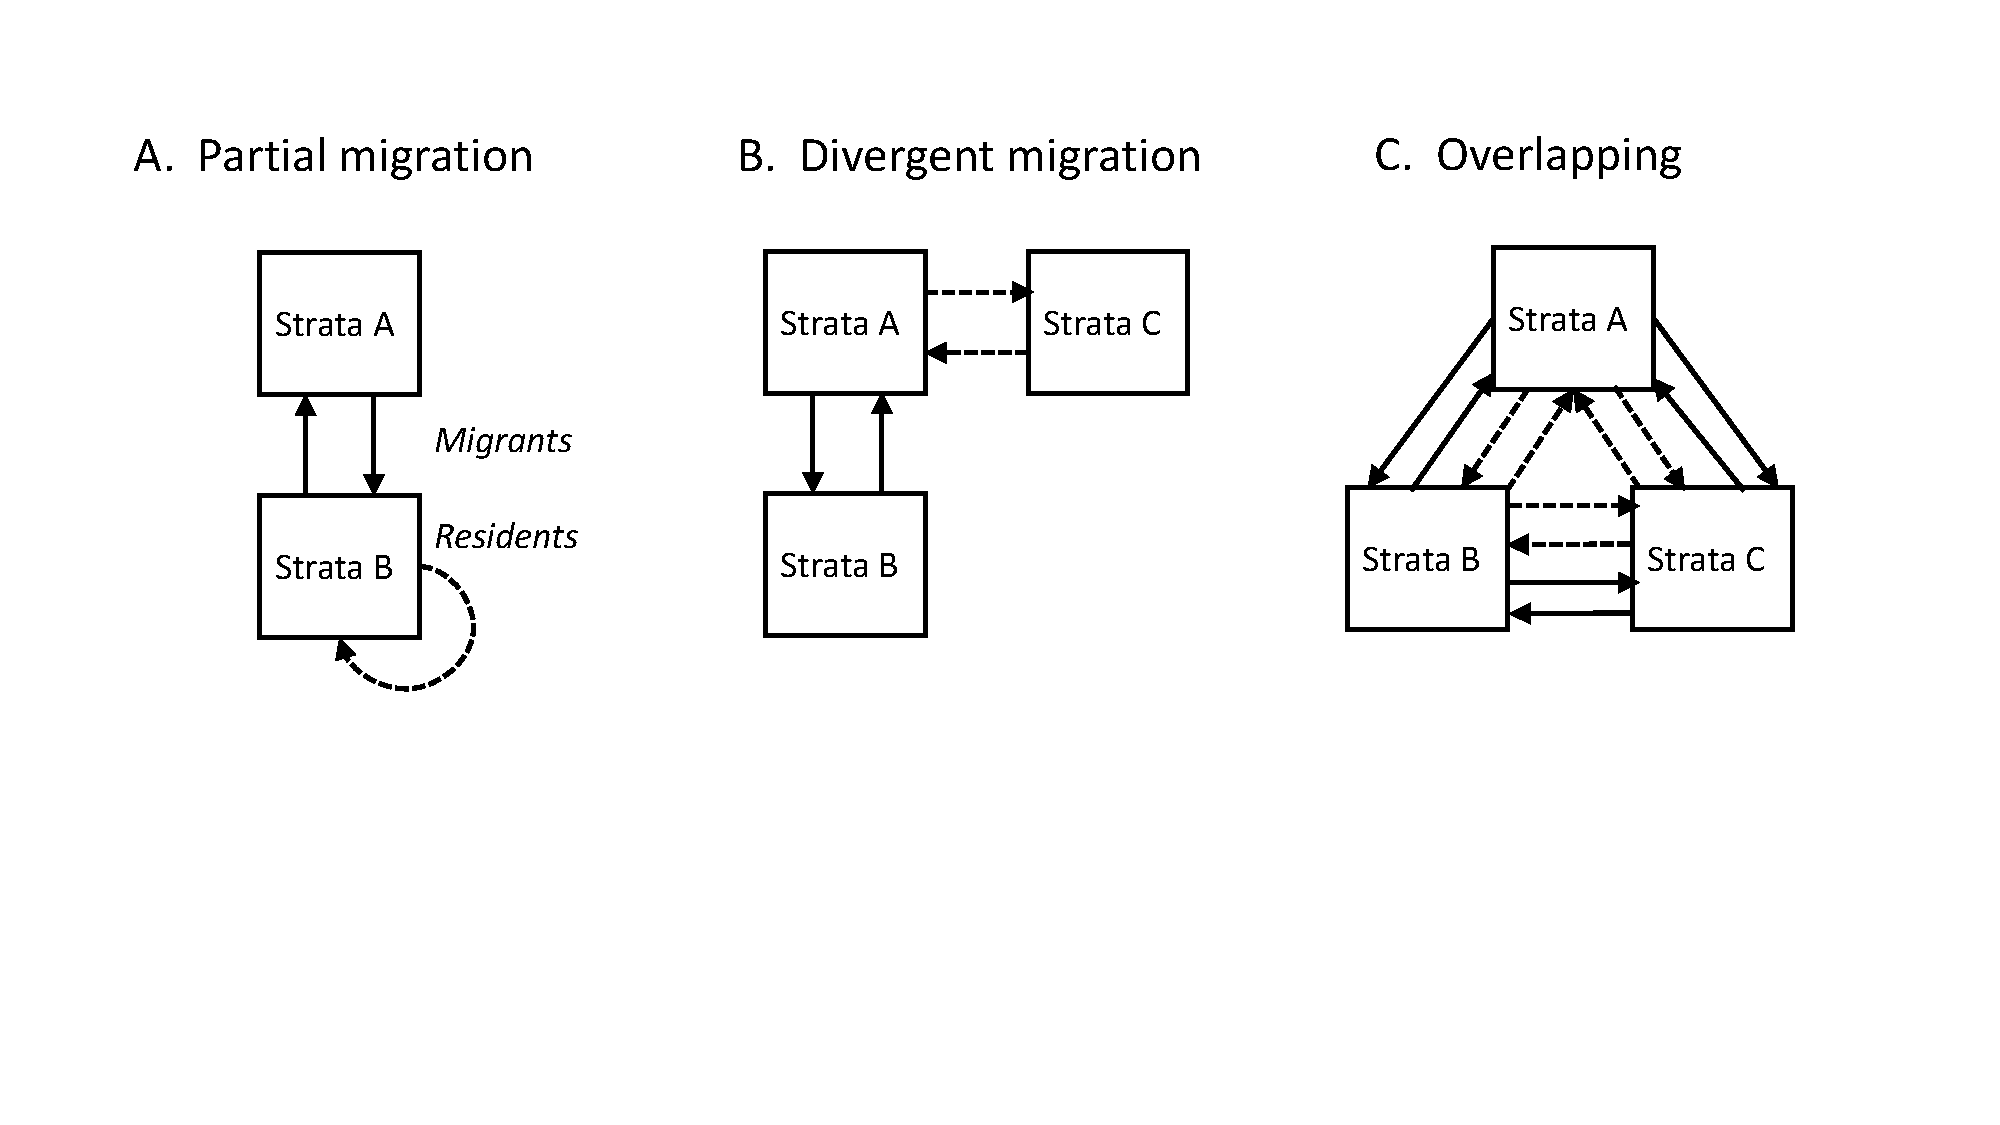
\includegraphics[width=170mm]{migration_diagrams.pdf}
\caption{A depiction of alternate movement patterns examined in simulation study of multistate mixture model performance. Each scenario uses two mixtures (subpopulations), each of which subscribe to a different migration/movement strategy.  In partial migration (A), residents stay in the same strata throughout the study, while migrants move seasonally (as with many waterfowl and songbird populations).  In divergent migration (B), animals of both subpopulations share a common strata (e.g. wintering area) at one time of the year, but move seasonally to different strata (e.g. summering areas).  In the overlapping scenario (C), animals of both subpopulations all make use of three different strata, but have preferences for different areas.   Subpopulation membership of each animal is assumed unknown at the time of marking.} \label{fig:migration}
\end{center}
\end{figure*}





\end{document}

%http://www.plosone.org/article/info:doi/10.1371/journal.pone.0036527
